\documentclass{standalone}
\usepackage{tikz}
\begin{document}
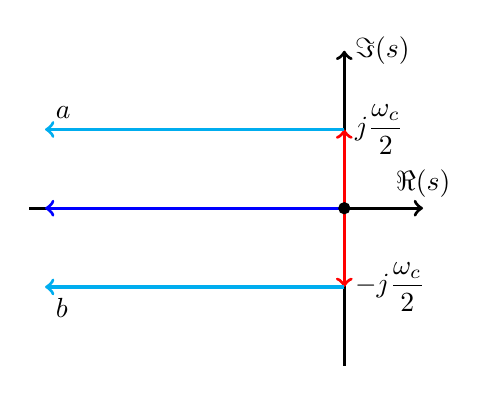
\begin{tikzpicture}[scale=2]
    \draw[->,very thick](-2,0)--(0.5,0)node[above]{$\Re(s)$};
    \draw[->,very thick](0,-1)--(0,1)node[right]{$\Im(s)$};

    \draw[->,very thick, red](0,0)--(0,0.5)node[right,black]{$\displaystyle j\frac{\omega_c}{2}$};       
    \draw[->,very thick, red](0,0)--(0,-0.5)node[right,black]{$\displaystyle-j\frac{\omega_c}{2}$};
    
    \draw[->,very thick,cyan](0,0.5)--(-1.9,0.5)node[above right,black]{$a$};
    \draw[->,very thick,cyan](0,-0.5)--(-1.9,-0.5)node[below right,black]{$b$};

    \draw[->,very thick, blue](0,0)--(-1.9,0);

    \filldraw[black](0,0)circle(1pt);
\end{tikzpicture}
\end{document}